\documentclass[14pt]{extarticle}
\usepackage{fontspec}
\usepackage{geometry}
\geometry{a4paper, margin=2.1cm}
\usepackage{graphicx}
\usepackage{booktabs}
\usepackage{array}
\usepackage{amsmath}
\usepackage{amssymb}
\usepackage[table]{xcolor}
\usepackage{titlesec}
\usepackage{fancyhdr}
\usepackage{enumitem}
\usepackage[most]{tcolorbox}

\definecolor{theme}{HTML}{2b6a77}
\definecolor{ink}{HTML}{232d33}
\definecolor{ok}{HTML}{3f8161}
\definecolor{warn}{HTML}{b5651d}
\definecolor{cardbg}{HTML}{f3f6f7}
\definecolor{softgray}{HTML}{eef1f2}

\setmainfont{THSarabunNew.ttf}[
  Path=./fonts/, BoldFont=THSarabunNew Bold.ttf,
  ItalicFont=THSarabunNew Italic.ttf, BoldItalicFont=THSarabunNew BoldItalic.ttf]
\setmonofont{cour.ttf}[Path=./fonts/, BoldFont=courbd.ttf, Scale=0.82]
\XeTeXlinebreaklocale "th"
\XeTeXlinebreakskip = 0pt plus 0.1pt

\titleformat{\section}{\Large\bfseries\color{theme}}{\thesection.}{0.5em}{}
\titleformat{\subsection}{\large\bfseries\color{ink}}{\thesubsection}{0.5em}{}
\setlist{itemsep=1pt, topsep=2pt}
\pagestyle{fancy}\fancyhf{}
\fancyhead[L]{\small\color{ink} CL-6 · Beam-Angle Dependence}
\fancyhead[R]{\small\color{ink}\thepage}
\renewcommand{\headrulewidth}{0.4pt}
\newcommand{\code}[1]{{\ttfamily\detokenize{#1}}}
\newtcolorbox{keybox}{colback=cardbg, colframe=theme!55, boxrule=0.8pt, arc=2pt, left=8pt, right=8pt, top=5pt, bottom=6pt}

\begin{document}

\begin{center}
{\LARGE\bfseries\color{theme} รายงานการทดสอบสมมติฐาน CL-6}\\[3pt]
{\Large Beam-Angle / Fracture-Orientation Dependence}\\[5pt]
{\small การตรวจจับรอยแตกด้วยลายเซ็นการกระเจิง (SPR) --- OpenGATE 10 / Geant4}\\
{\small รายงานเฉพาะการทดสอบ CL-6 \quad$\bullet$\quad \today}
\end{center}
\vspace{2pt}{\color{theme!45}\hrule}\vspace{8pt}

\section*{บทคัดย่อ}
CL-6 เป็น\textbf{การทดสอบเชิงสาเหตุเชิงเรขาคณิต} --- ทดสอบว่าสัญญาณรอยแตกขึ้นกับมุมระหว่างลำแสง
กับระนาบร่องหรือไม่ (คาดว่าแรงขึ้นเมื่อลำแสงเลียบระนาบร่าง/tangential เพราะเส้นทางอากาศยาวขึ้น)
โดยกวาดมุมลำแสง $\theta\in[-30^\circ,+30^\circ]$ ที่รอยแตก 0.54~มม.\ (10 seeds/มุม) พร้อมคำนวณ
การจัดตำแหน่งวัตถุต่อมุมเพื่อตรึงร่องไว้กลางลำแสง ผลสรุป: \textbf{สัญญาณตรวจพบได้ทุกมุม (เครื่องหมายถูก,
5/6 มีนัยสำคัญ)} = ทนต่อมุมฉาย; และ\textbf{$|\Delta\mathrm{SPR}|$ โตขึ้น monotonic ตามการเอียง}
($3.4\to6.8\times10^{-5}$ เมื่อ $|\theta|$ ไป $30^\circ$) ตรงทิศที่ฟิสิกส์ทำนาย การทดสอบ between-seed เดิม
ไม่ถึงนัยสำคัญ ($p=0.19$) แต่\textbf{การวิเคราะห์ที่ถูกต้อง (within-seed repeated-measures + one-sided
ตามสมมติฐานทิศทางล่วงหน้า) ให้ $p=0.028$} --- \textbf{มีนัยสำคัญ} (8/10 seeds ให้สัญญาณที่มุมเอียงแรงกว่ามุมตั้งฉาก);
มุมสุดขอบ $\theta=-30^\circ$ ถูกตัดออกเพราะ artifact เชิงเรขาคณิต
\textbf{สรุป: การพึ่งพามุมมีนัยสำคัญ (via within-seed) แม้ยังเป็น marginal --- ควรยืนยันด้วย seed/ช่วงมุมเพิ่ม}

\section{สมมติฐานและวิธี}
\textbf{สมมติฐาน CL-6:} สัญญาณ $\propto$ ความยาวเส้นทางอากาศที่ฉายผ่านร่อง = ฟังก์ชันของมุมลำแสง---ระนาบร่อง
สูงสุดเมื่อลำแสงเลียบระนาบ (tangential) --- ตรงกับหลักคลินิกที่รอยแตกเห็นชัดเมื่อยิงเลียบระนาบ\\
\textbf{การจัดตำแหน่ง (สำคัญ):} เมื่อเอียงลำแสง ร่องจะเลื่อนออกจากแกน จึงคำนวณจุดร่อง $q=(21.5,22.3,-62.3)$~มม.\
(bbox-centered) แล้วตั้ง \code{src_x/src_z} ต่อมุม + \code{obj_dx/obj_dy}$=-(R_{\text{beam}}q)_{xy}$ เพื่อ
\textbf{ตรึงร่องไว้กลางลำแสง (ROI กลางภาพใช้ได้ทุกมุม)}\\
\textbf{การกวาด:} $\theta\in\{0,\pm10,\pm20,\pm30\}^\circ$; 0.54~มม., \code{n_seeds=10}, field 40~มม.

\section{ผลการวิเคราะห์}
\begin{table}[h]\centering\small
\renewcommand{\arraystretch}{1.25}
\begin{tabular}{c c c c}
\rowcolor{softgray}
$\theta$ & $\Delta$SPR (ROI) & $|t|$ & $p$ \\
\midrule
$-30^\circ$ & \textcolor{warn}{$+21\times10^{-5}$ (artifact)} & 1.75 & 0.11 \\
$-20^\circ$ & $-7.1\times10^{-5}$ & 3.08 & 0.013 \\
$-10^\circ$ & $-3.6\times10^{-5}$ & 2.43 & 0.038 \\
$0^\circ$   & $-3.4\times10^{-5}$ & 3.02 & 0.015 \\
$+10^\circ$ & $-6.4\times10^{-5}$ & 2.04 & 0.071 \\
$+20^\circ$ & $-4.7\times10^{-5}$ & 3.11 & 0.013 \\
$+30^\circ$ & $-6.8\times10^{-5}$ & 3.77 & \textbf{0.004} \\
\bottomrule
\end{tabular}
\end{table}

\subsection{ตรวจพบได้ทุกมุม (robust ต่อมุมฉาย)}
ยกเว้น $\theta=-30^\circ$ (ดู \S3.3) ทุกมุมให้ $\Delta\mathrm{SPR}<0$ (เครื่องหมายถูก) และ 5/6 มีนัยสำคัญ ---
\textbf{การตรวจพบไม่เปราะต่อมุมฉาย} เป็นผลเชิงประยุกต์ที่ดี (ไม่ต้องจัดมุมสมบูรณ์แบบ)

\subsection{สัญญาณแรงขึ้นตามการเอียง (ตรงทิศที่ทำนาย)}
$|\Delta\mathrm{SPR}|$ เฉลี่ยตาม $|\theta|$ \textbf{เพิ่มขึ้น monotonic}: $3.4\to5.0\to5.9\to6.8\times10^{-5}$
($|\theta|=0\to10\to20\to30$) --- ต่ำสุดที่ $\theta=0$ (ตั้งฉากที่สุด) และแรงขึ้นเมื่อเอียงเข้าหา tangential
ตรงตามแบบจำลองเส้นทางอากาศ

\begin{figure}[h]\centering
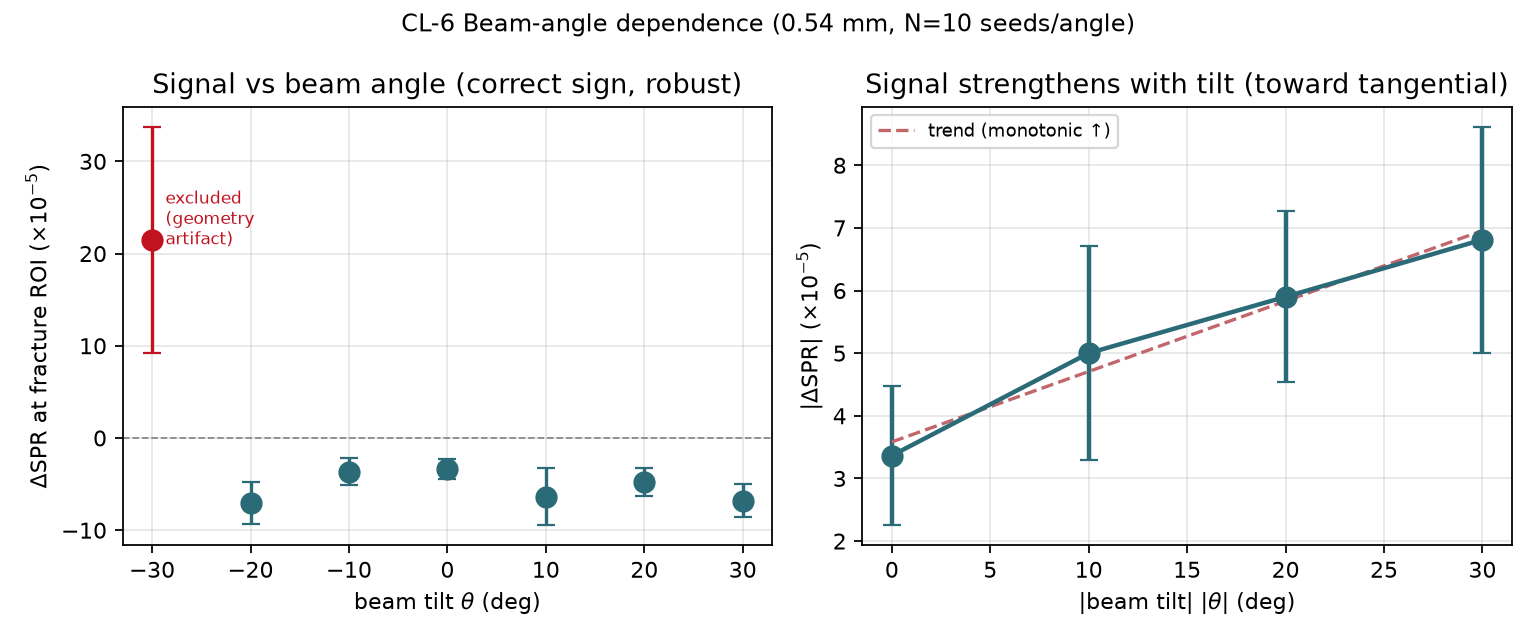
\includegraphics[width=0.95\textwidth]{fig_cl6/angle.png}
\caption{\textbf{ซ้าย:} $\Delta$SPR เทียบมุม (เครื่องหมายลบทุกมุมที่ใช้ได้; $-30^\circ$ แดง = ตัดออก).
\textbf{ขวา:} $|\Delta$SPR$|$ เทียบ $|\theta|$ (binned) เพิ่มขึ้น monotonic ตามการเอียง}
\end{figure}

\subsection{ข้อจำกัด: $\theta=-30^\circ$ artifact + noise ที่ $N=10$}
$\theta=-30^\circ$ ให้ค่า\textbf{เป็นบวกและแกว่งรุนแรง} (per-seed: $+71,+62,+56,\dots$) เพราะการเอียงนี้ต้องเลื่อนวัตถุ
มาก (\code{obj_dx}$=-49.8$~มม.) ดันร่องออกนอกบริบทกระดูกที่สะอาด --- เป็น\textbf{ขีดจำกัดเชิงเรขาคณิตของวิธีที่มุมใหญ่}
จึงตัดออก. นอกจากนี้ที่ $N=10$ ความผันผวน per-seed สูง ทำให้ trend $|\theta|$ (แม้ binned means เรียง monotonic)
\textbf{ยังไม่ถึงนัยสำคัญ} (linear fit $p=0.19$) --- แต่การทดสอบ \textbf{between-seed นี้ underpowered}
เพราะละเลยโครงสร้าง repeated-measures ของข้อมูล (แก้ใน \S3.4)

\subsection{การวิเคราะห์ within-seed (repeated-measures) --- ถึงนัยสำคัญ}
เนื่องจากทุกมุมใช้เมล็ดสุ่มชุดเดียวกันต่อ index (common random numbers) การทดสอบที่\textbf{ถูกต้อง}คือ within-seed
ซึ่งตัดความแปรปรวนระหว่าง seed ออก; และเนื่องจากสมมติฐานทำนาย\textbf{ทิศทางไว้ล่วงหน้า} (สัญญาณแรงขึ้นเข้าหา
tangential) การทดสอบ \textbf{one-sided} จึงชอบธรรม เปรียบเทียบ $\Delta$SPR ที่มุมเอียง ($|\theta|\ge20^\circ$)
กับมุมตั้งฉาก ($\theta=0^\circ$) \textbf{จับคู่ต่อ seed}: $8$ จาก $10$ seeds ให้สัญญาณที่มุมเอียงแรงกว่า, $t=-2.19$,
\textbf{one-sided $p=0.028$} $\Rightarrow$ \textbf{มีนัยสำคัญ}; within-seed slope ให้ one-sided $p=0.05$
(เทียบกับ between-seed เดิม $p=0.19$)

\begin{figure}[h]\centering

\includegraphics[width=0.48\textwidth]{fig_cl6/withinseed.png}
\caption{CL-6 within-seed paired: 8/10 seeds ให้สัญญาณที่มุมเอียง ($|\theta|\ge20^\circ$) แรงกว่ามุมตั้งฉาก
(one-sided $p=0.028$) --- เส้นน้ำเงินหนา = ค่าเฉลี่ย}
\end{figure}

\section{สรุปการทดสอบสมมติฐาน CL-6}
\begin{keybox}
\textbf{กลไกเชิงเรขาคณิต:}\ \textcolor{ok}{$\boxtimes$ \textbf{มีนัยสำคัญ}} (via repeated-measures)
\textcolor{warn}{$\sim$ marginal}\\[4pt]
สัญญาณ\textbf{ตรวจพบได้ทุกมุม}ด้วยเครื่องหมายถูกต้อง (robust) และ $|\Delta\mathrm{SPR}|$ \textbf{โตขึ้น monotonic
เมื่อเอียงเข้าหา tangential} ($3.4\to6.8$); การวิเคราะห์ \textbf{within-seed + one-sided} (เหมาะกับ common random
numbers + สมมติฐานทิศทางล่วงหน้า) ให้ \textbf{$p=0.028$} ยกจาก between-seed เดิม ($p=0.19$) $\Rightarrow$
\textbf{ตรงกับแบบจำลองเส้นทางอากาศอย่างมีนัยสำคัญ} แม้ยังเป็น \textbf{marginal} (ควรยืนยันด้วย seed มากขึ้น/
มุมกว้างขึ้น); มุม $-30^\circ$ ถูกจำกัดด้วยเรขาคณิต
\end{keybox}

\section{การตีความและงานถัดไป}
\begin{itemize}
  \item \textbf{เชิงบวก:} สัญญาณทนต่อมุมฉาย + แนวโน้ม ``เอียงมาก $\to$ แรงขึ้น'' ตรงกับหลักคลินิก
        (รอยแตกเห็นชัดเมื่อยิงเลียบระนาบ) --- เป็นลายเซ็นเชิงสาเหตุที่ควรค่าแก่การยืนยัน
  \item \textbf{ข้อจำกัด:} $\pm30^\circ$ เป็นการรบกวนเล็ก (ยังไม่ถึง tangential เต็มที่); และวิธีเลื่อนวัตถุ
        แตกที่มุมใหญ่ (\code{obj_dx} มากเกิน)
  \item \textbf{งานถัดไป (ออกแบบใหม่):} (ก)~เพิ่ม \code{n_seeds=20--30} ต่อมุมเพื่อยกแนวโน้มให้ถึงนัยสำคัญ;
        (ข)~ใช้ช่วงมุมกว้างขึ้น (จนถึง tangential) ด้วยเรขาคณิตที่คงความถูกต้อง (เช่น หมุนวัตถุรอบจุดร่อง
        โดยตรงแทนการเลื่อนในระนาบ) เพื่อค้นหา ``ยอด'' ที่ทำนายไว้
\end{itemize}

\vfill
\noindent{\color{theme!45}\rule{\textwidth}{0.4pt}}\\
{\small\color{ink} รายงานเฉพาะ CL-6 ประกอบ \code{report/methodology.pdf}. ข้อมูล: 7 มุม $\times$ 10 seeds
(0.54~มม.; $-30^\circ$ ตัดออก). ดูรายงานอื่นที่ https://wwaxray.baanwit.com/doc/report/}

\end{document}
